\documentclass[11pt]{article}
\usepackage{enumitem}
\usepackage{tikz}
\usetikzlibrary{automata, positioning}
\usepackage{latexsym}
\usepackage{amsfonts}
\usepackage{amsmath,amssymb,amsthm}
\usepackage{xcolor}
\usepackage{multicol}

\usepackage{tikz}
\usetikzlibrary{arrows}
\usetikzlibrary{automata}

\setlength{\textheight}{8.5in}
\setlength{\textwidth}{6.0in}
\setlength{\headheight}{0in}
\addtolength{\topmargin}{-.5in}
\addtolength{\oddsidemargin}{-.5in}

\input{preamble.tex}

\newcommand{\solution}[1]{\paragraph{Solution}  }

\begin{document}
\exam{1: Regular Languages}{Due: 12:30 pm Feb 20}{Released: 12:30 pm Feb 19}{}

This exam was released at 12:30 pm EST Thursday, February 19, and is due at \textbf{12:30 pm EST on Friday, February 20}. There are no late submissions; leave yourself enough time to upload your work.

You should submit a typeset or \emph{neatly} written pdf on Gradescope.  The grading TA should not have to struggle to read what you've written; we can't give points to an answer that we can't read.

Enter your work using the \verb|answer| environment we have provided for you. The default color is \textcolor{teal}{teal}, but you can choose to change it to any of \textcolor{red}{red}, \textcolor{brown}{brown}, \textcolor{magenta}{magenta}, \textcolor{violet}{violet}, \textcolor{blue}{blue}, \textcolor{darkgray}{darkgray}, or black like so:
\begin{verbatim}
                        \begin{answer}[<COLOR>]
                            <YOUR WORK GOES HERE> 
                        \end{answer}
\end{verbatim}

This exam is open book and open notes. However, you may \textbf{NOT} use the internet to look up answers, and you may \textbf{NOT} discuss the exam with your fellow students or anyone else besides the TA's and the professor before the exam is due.

If you have questions during the exam, there will be a pinned thread on Piazza monitored by the TA's.
\begin{enumerate}

\item[0.] \textbf{Honor Code} 1 point

I commit to uphold the ideals of honor and integrity by refusing to betray the trust bestowed upon me as a member of the Georgia Tech community.

Signature: Aamod Varma  %\hrulefill

\item \textbf{Short Answer} 6 points

\begin{enumerate}
    
    
    \item (2 points) Suppose you are trying to prove that $L = \{ww\ |\ w \in \Sigma^*\}$ is not regular using the pumping lemma. You have already assumed that $L$ is regular, and let $p$ be the pumping length. Explain why the string $1^p1^p$ \textbf{cannot} be used as a choice for $s$ that will lead to a contradiction. 
    
      \begin{answer}
      In the pumping lemma we write a string $s = xyz$ so if we take $1^{p}1^{p} = xyz$ then we need $|xy| \le p$ and $|y| > 0$. This means we have $xy$ a substring of $1^{p}$. So let $x = 1^{m}$ and $y = 1^{n}$ where $m + n$ where $m + n \le p$ and $n > 0$. Now note that is' enough to show that there exists one decomposition in which all $i$ keep the string $xy^{i}z$ in $L$. Now consider the case where $x = \epsilon, y = 1^2, z= 1^{2p - 2}$. Now note that in this case we have $$xy^{i}z = 1^{2i}1^{2p - 2} = 1^{2(p + i - 1)}= w w$$ where $w = 1^{p + i - 1}$, in other words we have $xy^{i}z \in L$ for all $i$. Clearly this means that we cannot use this as a contradiction. In essence, there is a valid decomposition that does not produce a contradiction.
    \end{answer}
    
    \item (2 points - \textit{Section B only}) 
   Give some example regular language $L$ crafted from $A$ and $B$ and $C$ such that $AB\cup C$ is $L$ but $A$ and $B$ and $C$ are each not regular. State what $A$, $B$, $C$ and $L$ represent in your specific example. 
    
    \begin{answer}
        % Enter your work here
    \end{answer}
    
    \item (2 points - \textit{Section X only}) Let $L$ be a regular language, and let $D$ be a DFA for $L$ with $q$ states. Show that one of the following must be true:
    \begin{itemize}
    \item $L$ contains infinitely many strings
    
    \begin{answer}

      Consider the case where we have a loop in the DFA $D$ that is in an accepting path. That is there exists some state $q_i$ for which there is a string $s_{0}$ that can traverse from the start state $q_0$ to $q_i$, a string $s_{1}$ that is not the empty string that loops from $q_i$ to itself and a string $s_{2}$ that goes from $q_i$ to the accept state. Clearly $s_{0}s_{1}s_{2}$ is a string accepted by this language. But now note that we can loop arbitrarily many times to create an infinite number of strings. More specifically any string $s_{0}s_{1}^{i}s_{2}$ for $i \in N \ge 0$ is a string accepted by our language. Now as all these strings for the varying $i$ are distinct we have an infinite number of strings that are accepted by  $D$. 

    \end{answer}
    
    \item $L$ contains only strings of length less than or equal to $q-2$.
    
    \begin{answer}
      On the contrary assume there is no cycle in our DFA on any accepting path, this means that for any string that is accepted by our language, no state in that has a loop to itself. But this means that it's only possible to visit a state once in this path. Now note that if $D$ has $q$ states, then the maximum number of states that can be included in an accepting string is $q - 1$ states, this is because as each state is defined for a specific alphabet, that means even the accepting state needs to have an outgoing transition, if it transitions to any of the previous $q - 1$ states including itself then we have a cycle, so it must point to another state that cannot join back to the initial $q - 1$ states. Once we're in this sink state, we must not be able to become an accepting string. Hence we can have a maximum of $q - 1$ states in the accepting path. But $q - 1$ states have $q - 2$ edges or transitions. Hence the longest string we can have is $q - 2$.
    \end{answer}
    
    \end{itemize}
\end{enumerate}


\item \textbf{Nondeterminism} 6 points

Let $L^R = \{ w^R | w \in L\}$, i.e. the set of strings which are the reverse of some string in $L$. Show by constructing an NFA that if $L$ is a regular language, then $L^R$ is also regular.


\begin{answer}
  Let $M$ be the DFA of $L$, we need to show that there exists a NFA that accepts $L^{R}$. Now we construct our NFA $N$ by first copying over the DFA of $L$ and modifying it as follows, 
  \begin{enumerate}
    \item First we reverse each transition. For any $\delta_M(q, \alpha) = p$ we have $\delta_N(p, \alpha) = q$.
    \item We define the accept state of our NFA as the start state of our DFA. So our accept state in $N$ is just $\{q_{0}\}$ where $q_{0}$ is the start state of the DFA.
    \item We define a new start state in $N$ called $q'$ and we add $\epsilon-$transitions to all the accepts states in the previous DFA. i.e for all $q \in F$ we have $\delta_N(q', \epsilon) = q$.
  \end{enumerate}

  Now let $s$ be a string in $L$ represented as $s = x_{1} \dots x_n$. Now clearly $x_{1} \dots x_n$ is accepted by $M$. I.e we have a sequence of states $q_0, \dots, q_m$ such that $q_0$ is the start state $q_m$ is the accept state and $\delta_M(q_i, x_j) = q_{i + 1}$. Now note that in our NFA $N$ we have $q'$ as our start state that has an $\epsilon$ transition to each accept state of $M$  which includes $q_m$. So if we consider the string $s' = x_n \dots x_1$ in our NFA $N$ note that we have for every $\delta_M(q_i, x_j) = q_{i + 1})$ that $\delta_N(q_{i + 1}, x_j) = q_i$ hence we take the exact reverse direction until we reach $\delta_N(q_1, x_q) = q_0$ but note $q_0$ in $N$ is defined as our accept state. Hence we have $x_m \dots x_1$is accepted by our NFA. Similarly if $N$ accepts a string $s$ then reversing the accepting path gives a path in our DFA $M$ which would accept $w^{R}$ and hence we have $w \in L^{R}$.
\end{answer}

\item \textbf{Regular expressions} 6 points

(3 points) 
Give an equivalent NFA for the following expression: $1(010)^*(1(10)^* \cup 00)^*1$

\begin{answer}
  \vspace{1em}
  \begin{center}
    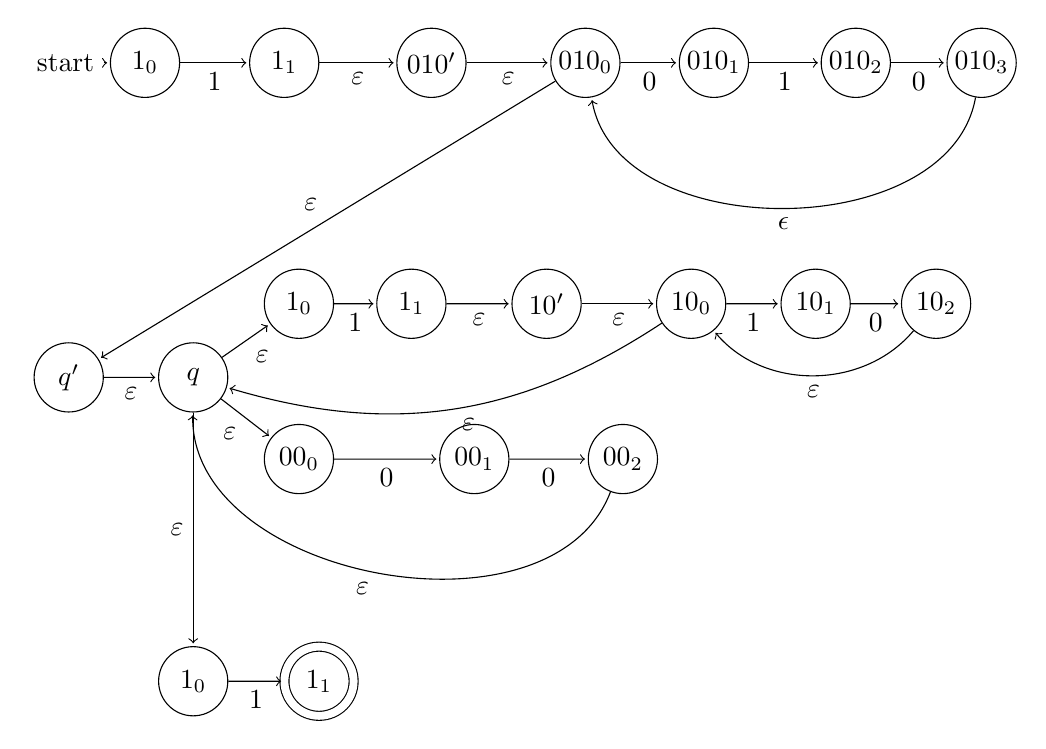
\begin{tikzpicture}[shorten >=1pt,node distance=2cm,on grid,auto,scale=0.17]
\tikzset{accepting/.style={double distance=1mm}}
\node[state,initial, label=center:{$1_0$}] (0) at (10.6,-8.6) {};
\node[state, label=center:{$1_1$}] (1) at (21,-8.6) {};
\node[state, label=center:{$010_0$}] (2) at (43.5,-8.6) {};
\node[state, label=center:{$010_1$}] (3) at (53.1,-8.6) {};
\node[state, label=center:{$010_2$}] (4) at (63.7,-8.6) {};
\node[state, label=center:{$010_3$}] (5) at (73.1,-8.6) {};
\node[state, label=center:{$10_0$}] (6) at (51.4,-26.6) {};
\node[state, label=center:{$10_1$}] (16) at (60.7,-26.6) {};
\node[state, label=center:{$10_2$}] (17) at (69.7,-26.6) {};
\node[state, label=center:{$10'$}] (18) at (40.6,-26.6) {};
\node[state, label=center:{$1_0$}] (19) at (22.1,-26.6) {};
\node[state, label=center:{$1_1$}] (20) at (30.5,-26.6) {};
\node[state, label=center:{$00_0$}] (21) at (22.1,-38.2) {};
\node[state, label=center:{$00_1$}] (22) at (35.2,-38.2) {};
\node[state, label=center:{$00_2$}] (23) at (46.3,-38.2) {};
\node[state, label=center:{$1_0$}] (24) at (14.2,-54.8) {};
\node[state,accepting, label=center:{$1_1$}] (25) at (23.6,-54.8) {};
\node[state, label=center:{$010'$}] (26) at (32,-8.6) {};
\node[state, label=center:{$q$}] (28) at (14.2,-32.1) {};
\node[state, label=center:{$q'$}] (31) at (4.9,-32.1) {};
\path[->] (0) edge node [swap] {$1$} (1);
\path[->] (3) edge node [swap] {$1$} (4);
\path[->] (2) edge node [swap] {$0$} (3);
\path[->] (4) edge node [swap] {$0$} (5);
\path[->] (16) edge node [swap] {$0$} (17);
\path[->] (18) edge node [swap] {$\varepsilon$} (6);
\path[->] (6) edge node [swap] {$1$} (16);
\path[->] (19) edge node [swap] {$1$} (20);
\path[->] (21) edge node [swap] {$0$} (22);
\path[->] (22) edge node [swap] {$0$} (23);
\path[->] (24) edge node [swap] {$1$} (25);
\path[->] (26) edge node [swap] {$\varepsilon$} (2);
\path[->] (5) edge[bend left=80 ] node {$\epsilon$} (2);
\path[->] (1) edge node [swap] {$\varepsilon$} (26);
\path[->] (17) edge[bend left=50 ] node {$\varepsilon$} (6);
\path[->] (20) edge node [swap] {$\varepsilon$} (18);
\path[->] (28) edge node [swap] {$\varepsilon$} (19);
\path[->] (28) edge node [swap] {$\varepsilon$} (21);
\path[->] (31) edge node [swap] {$\varepsilon$} (28);
\path[->] (23) edge[bend left=80 ] node {$\varepsilon$} (28);
\path[->] (6) edge[bend left=25 ] node {$\varepsilon$} (28);
\path[->] (2) edge node [swap] {$\varepsilon$} (31);
\path[->] (28) edge node [swap] {$\varepsilon$} (24);
\end{tikzpicture}

  \end{center}

\end{answer}

(3 points) 

Using an alphabet ($\Sigma$) of only lowercase vowels ('a', 'e', 'i', 'o', 'u'), give a regular expression representing all strings where 'a's cannot be the first or last letter. 

\begin{answer}
  
  So we need to start with other letters and end with other letters except $a$. So for the first letter we have $(e \cup i \cup o \cup u)$, the middle can be any letter so we have $(a \cup e \cup i \cup o \cup u)^*$ and the last letter is non-a as well which is, $(e \cup i \cup o \cup u)$ so putting it together we have, 
  \[
    (e \cup i \cup o \cup u)(a \cup e \cup i \cup o \cup u)^*(e \cup i \cup o \cup u)
  \]

  Now note that this implies our string is length 2 or above. So to include length 1 strings we have, 

  \[
    (e \cup i \cup o \cup u) \cup  (e \cup i \cup o \cup u)(a \cup e \cup i \cup o \cup u)^*(e \cup i \cup o \cup u)
  \]
\end{answer}


\item \textbf{Pumping lemma} 6 points

Use the pumping lemma to prove that $L =\{x\#y\#z \: | \: x \in \{0, 1\}^*, y \in \{0, 1\}^*, z \in \{0, 1\}^*, bin(x) * bin(y) = bin(z)\}$ is not regular. Here, $\Sigma = \{0, 1, \#\}$ and $bin(x)$ is the decimal value of $x$ when interpreted as a binary string. For example: $bin(101) = 5$. 

\begin{answer}
  Let $p$ be the pumping length, now consider the string $s = 10^{p}1\#1\#10^{p}1$. Note that we have $x = 10^{p}1, y = 1, z = 10^{p}1$. Clearly because $bin(y) = bin(1) = 1$ we trivially have $bin(x) * bin(y) = bin(x) = bin(z)$ as $x = z$. We also have $|s| \ge p$. Now if the language is regular  we can write it as $s = uvw$ where $|uv| \le p$ and $|v| > 0$  and for any $i \in N \ge 0$ we have $uv^{i}w \in L$. Now this means we have $10^{p}1 \# 1 \# 10^{p}1 = uvw$ but note if $|uv| \le p$ then $|uv|$ must be a prefix of $10^{p - 1}$ (note that $v$ cannot contain $\#$ as we can pump $v$ in the beginning of the string which in this case is the first $p$ letters and they don't contain $\#$, note that if it did contain $\#$ it's trivially a contradiction as we can pump it to any length and we now have more than 3 $\#$ which puts it outside the language). Now note that the possible decomposition we can have are,
  \begin{enumerate}
    \item $v$ contains the leading $1$ and hence is equal to $10^{k}$ for $1 \le k \le p - 2$ and $u = \epsilon$. Now in this case simply consider $i = 0$. This gives us the string $uv^{0}w = w = 0^{p - k}1\#1\#10^{p}1$. Clearly $bin(0^{k}1) * bin(1)  = bin(1)* bin(1) = 1 * 1= 1 \ne bin(10^{p}1)$.
    \item $v$ does not have the leading $1$ so it's just a bunch of zeroes so it is equal to $0^{k}$ for some $1 \le k \le p - 1$. Consider again $i = 0$, now we have $10^{p - k}1\# 1 \# 10^{p}1$. Now as $k \ge 1$ we cannot have $p - k = p$ so clearly the binary number $10^{p - k}1 \ne 10^{p}1$ and hence it is not true that $bin(10^{p - k}1) * bin(1) = bin(10^{p}1)$.
  \end{enumerate}

\end{answer}

\end{enumerate}
\end{document}
